\section{Exercise 4}

Consider the following network diagram:
\begin{figure}[H]
    \centering
    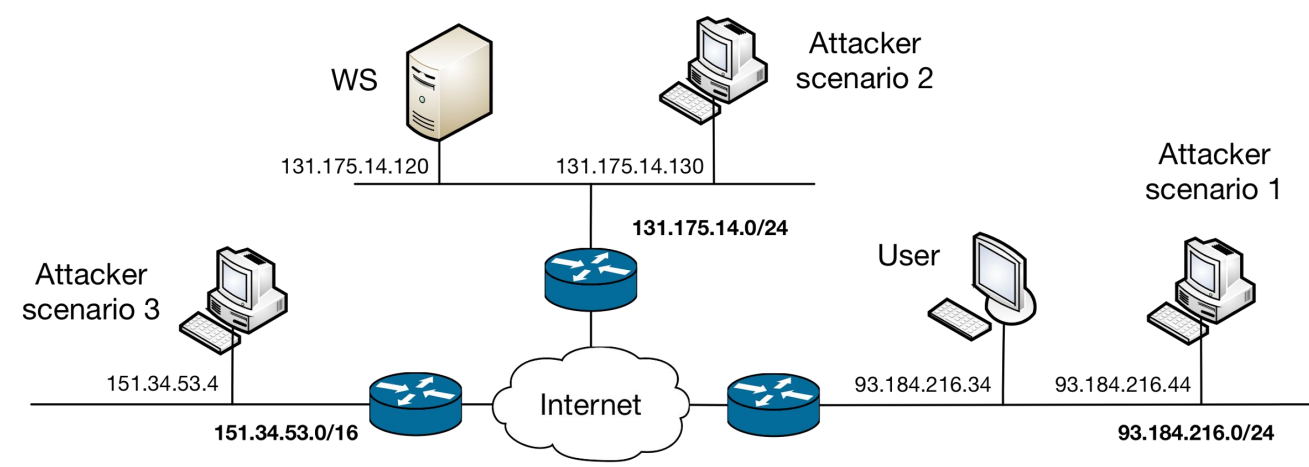
\includegraphics[width=0.75\linewidth]{images/net1.png}
\end{figure}
A user, with IP address 93.184.216.34, is attempting to download a software executable from a web server in the Politecnico di Milano network with IP address 131.175.14.120, over the HTTP protocol (no HTTPS, no signatures, nothing).
Assume that the user's browser already cached the IP address of downloads.polimi.it (i.e., it does not perform any DNS request), and that there is no firewall involved. 
An attacker, who knows that the user is about to download this software, wants to target our user by carrying out an attack to replace the downloaded software with a piece of malware.
For each of the following attack scenarios, state whether the attacker is able to fulfill his goals. 
If you deem it possible, describe an attack that allows to do so: state the name of the class of attacks, and describe all the steps needed to make it work in this specific scenarios. 
If multiple classes of attacks are possible, focus on the simplest one that gets the job done. 
If no attack is possible, please explain why.
\begin{enumerate}
    \item Attacker: 93.184.216.44; same network and broadcast domain of the user. 
    \item Attacker: 131.175.14.130; same network of web server, but different than user. 
    \item Attacker: 151.34.53.4; attacker, user and web server on three different networks. 
\end{enumerate}
For the next questions consider ONLY scenario 3. 
Assume that each involved computer and server implements a custom TCP/IP stack that, for performance reasons, sets the TCP initial sequence number in the SYN and SYN+ACK packets as the most significant bits of the current timestamp.
\begin{enumerate}
    \item [3. ] Describe the security issue with the proposed ISN implementation, and propose a way to solve the issue. 
    \item [4. ] Describe how the attacker can perform the above attack, this time exploiting the security issues raised by the custom ISN implementation. 
        Describe all the steps and assumptions that you need to perform this attack.
    \item [5. ] Assume you are the network security administrator of the network of the attacker (in the scenario 3 and assuming the custom TCP initial sequence number implementation), and that you control the border router between the network 151.34.53.0/24 and the rest of the Internet.
        Propose a way to prevent the attack. 
        Can the administrator of the other two border routers in the diagram deploy the same mitigation, and obtain the same result? Why?
\end{enumerate}

\subsection*{Solution}
\begin{enumerate}
    \item ARP spoofing. 
    \item ARP spoofing (but this time target the server). 
    \item No attack possible, because HTTP uses TCP and, if sequence numbers are correctly implemented, not possible to perform TCP hijacking. 
        Also, DNS poisoning not possible as DNS response already cached.
    \item Can predict ISN, so we can solve by using random ISN. 
    \item TCP hijacking. 
        We can guess the ISN of the SYN packet sent by the victim (the user), we can spoof the web server IP and send a correct SYN+ACK to it and, if we can guess the content of the request (we do), subsequent packets. 
        This way we can send a different payload. 
        In parallel we can also use TCP hijacking to send a fake RST to the actual server spoofing the user's IP address.
        Problem and assumption: we need to know the ephemeral port used by the client to initiate the connection. 
    \item We can filter the packets with source IPs not belonging to our network.
        Other routers can't do this, they can only filter out packets coming from outside with spoofed IPs belonging to their network, but it's of little use in this scenario.
\end{enumerate}